Čia yra literatūros apžvalga. Šitas mokslininkas padarė taip \cite{horvath2016}.
%
Kitas klausimas.

Toliau apžvelgsime \cite{ezhov1969} darbus.

https://machinelearningmastery.com/learning-rate-for-deep-learning-neural-networks/

Neuroniai tinklai arba kitaip dirbtinio intelekto neuroniai tinklai yra mašininio mokymo metodai, kurie leidžia kompiuteriui mokytis iš stebimų duomenų. Neuroninių tinklų veikimo principas yra įkvėptas pagal tai kaip biologinė nervų sistema apdoroja informaciją.\cite{Sukhadeve2017}

% Neuroninių tinklų sprendžiamos problemos

Esminis neuroninio tinklo elementas yra dirbtinis neuronas. Šį neuroną sudaro pagrindiniai trys komponentai: įvesties reikšmės, svoriai, kurie jungia šias reikšmes su neuronu ir aktyvacijos funkcija. Tai yra pats paprasčiausias neurono modelis, vadinamas Perceptronu (angl. \textit{Perceptron}).\cite{Andrew2017}

\begin{figure}
  \centering
\scalebox{0.5}{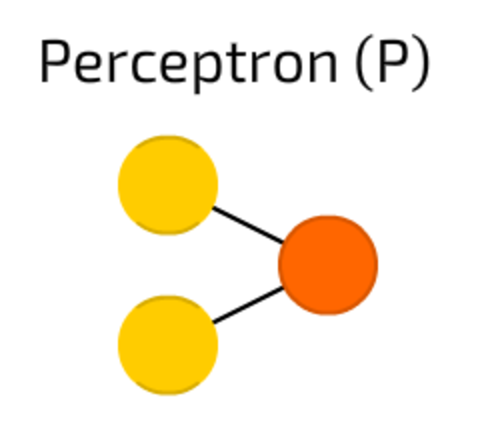
\includegraphics{images/perceptron.png}}
\caption{Testuojam jpg įtraukimą.}
\end{figure}

\begin{figure} \label{fig:perceptron}
  \centering
\scalebox{0.5}{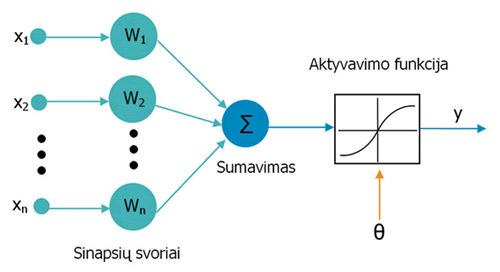
\includegraphics{images/perceptron_pvz.png}}
\caption{Dirbtinio neurono modelis (Perceptronas).}
\end{figure}

Paveiksle pavaizduoto Perceptrono reikšmė apskaičiuojama pagal formulę
\begin{equation*}
  y = f \left(\sum_{k=1}^{n} x_k W_k \right),
\end{equation*}

čia f - aktyvavimo funkcija.

Paveiksle \ref{fig:perceptron} pavaizduoto neurono veikimo principas:
\begin{enumerate}

\item Neuronas gauna įvesties reikšmes $x_1, x_2, ... , x_n$. Kiekviena iš reikšmių turi savo perdavimo koeficientą į neuroną (svorį) $W_1, W_2, ... , W_n$.
\item  Skaičiuojama įvesties reikšmių ir atitinkamų svorių sandaugų suma(žymima z):
  $z = \sum_{k=1}^{n} x_k * W_k$
\item  Neurono išvesties reikšmė(žymima a) yra apskaičiuojama įvesties reikšmių ir atitinkamų svorių sandaugų sumai pritaikius aktyvacijos funkciją(žymima f).
  $a = f(z) = f(\sum_{k=1}^{n} x_k * W_k)$
\end{enumerate}

\subsection{Sužadinimo signalai(angl. \textit{Bias neuron})}
Dažniausiai įvesties reikšmių yra vienetu daugiau, nei yra paduodama įvesties reikšmių. Ši įvestis yra vadinama sužadinimo signalu (angl. \textit{Bias neuron}). Šio signalo reikšmė yra pastovi ir visada lygi vienetui($x_{n+1} = 1$). Taip pat yra pridedamas papildomas svoris $W_{n+1}$ jungiantis šį signalą su neuronu.\cite{Ieva2012}
Šis sužadinimo signalas padeda lengvai koreguoti neurono išvesties reikšmę, kadangi įvesties reikšmė yra vienetas, tuomet sandauga, kuri yra prisumuojama priklauso tik nuo svorio jungiančio sužadinimo signalą su neuronu. Ji yra lygi  $W_{n+1}$. Naudojant sužadinimo signalus neuroniai tinklai yra daug sparčiau apmokinami, kadangi šie signalai gali laisvai koreguoti perduodamą reikšmę į neuronus.
  \subsection{Aktyvacijos funkcijos(angl. \textit{Activation function})}
Neurono išvesties reikšmei apskaičiuoti naudojamų aktyvacijos funkcijų yra visokiausių tipų.




Patys pirmieji neuroninio tinklo modeliai buvo sukurti Tiesioginio sklidimo (angl. \textit{Feed forward}) neuroniniai tinklai.

\cite{Ieva2012}


%padaryti feedforward vieno apskaiciavima
Šiuo būdu realizuoto neurononio tinklo schema pavaizduota (). Čia




\begin{figure}
  \centering
\scalebox{0.5}{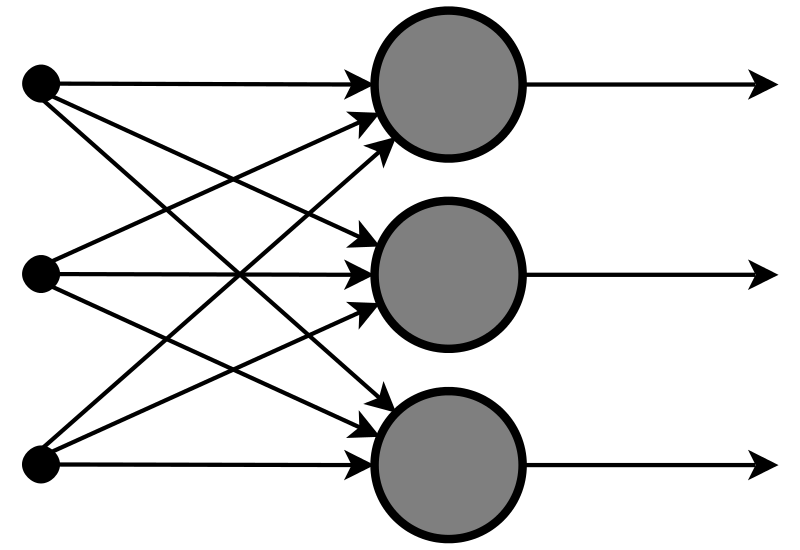
\includegraphics{images/feedforward.png}}
\caption{Testuojam jpg įtraukimą.}
\end{figure}



Dirbtinis intelektas


neuroniai tinklai, ju tipai


Neuroninių tinklų yra daug tipų, pagal



lstm neuroninis tinklas

taikymas language Modelling


Dirbtinis intelektas
